\documentclass{standalone}
\usepackage{tikz}
\usetikzlibrary{patterns, positioning}
\usepackage[sfdefault]{ClearSans} %% option 'sfdefault' activates Clear Sans as the default text font
\usepackage[T1]{fontenc}

\begin{document}
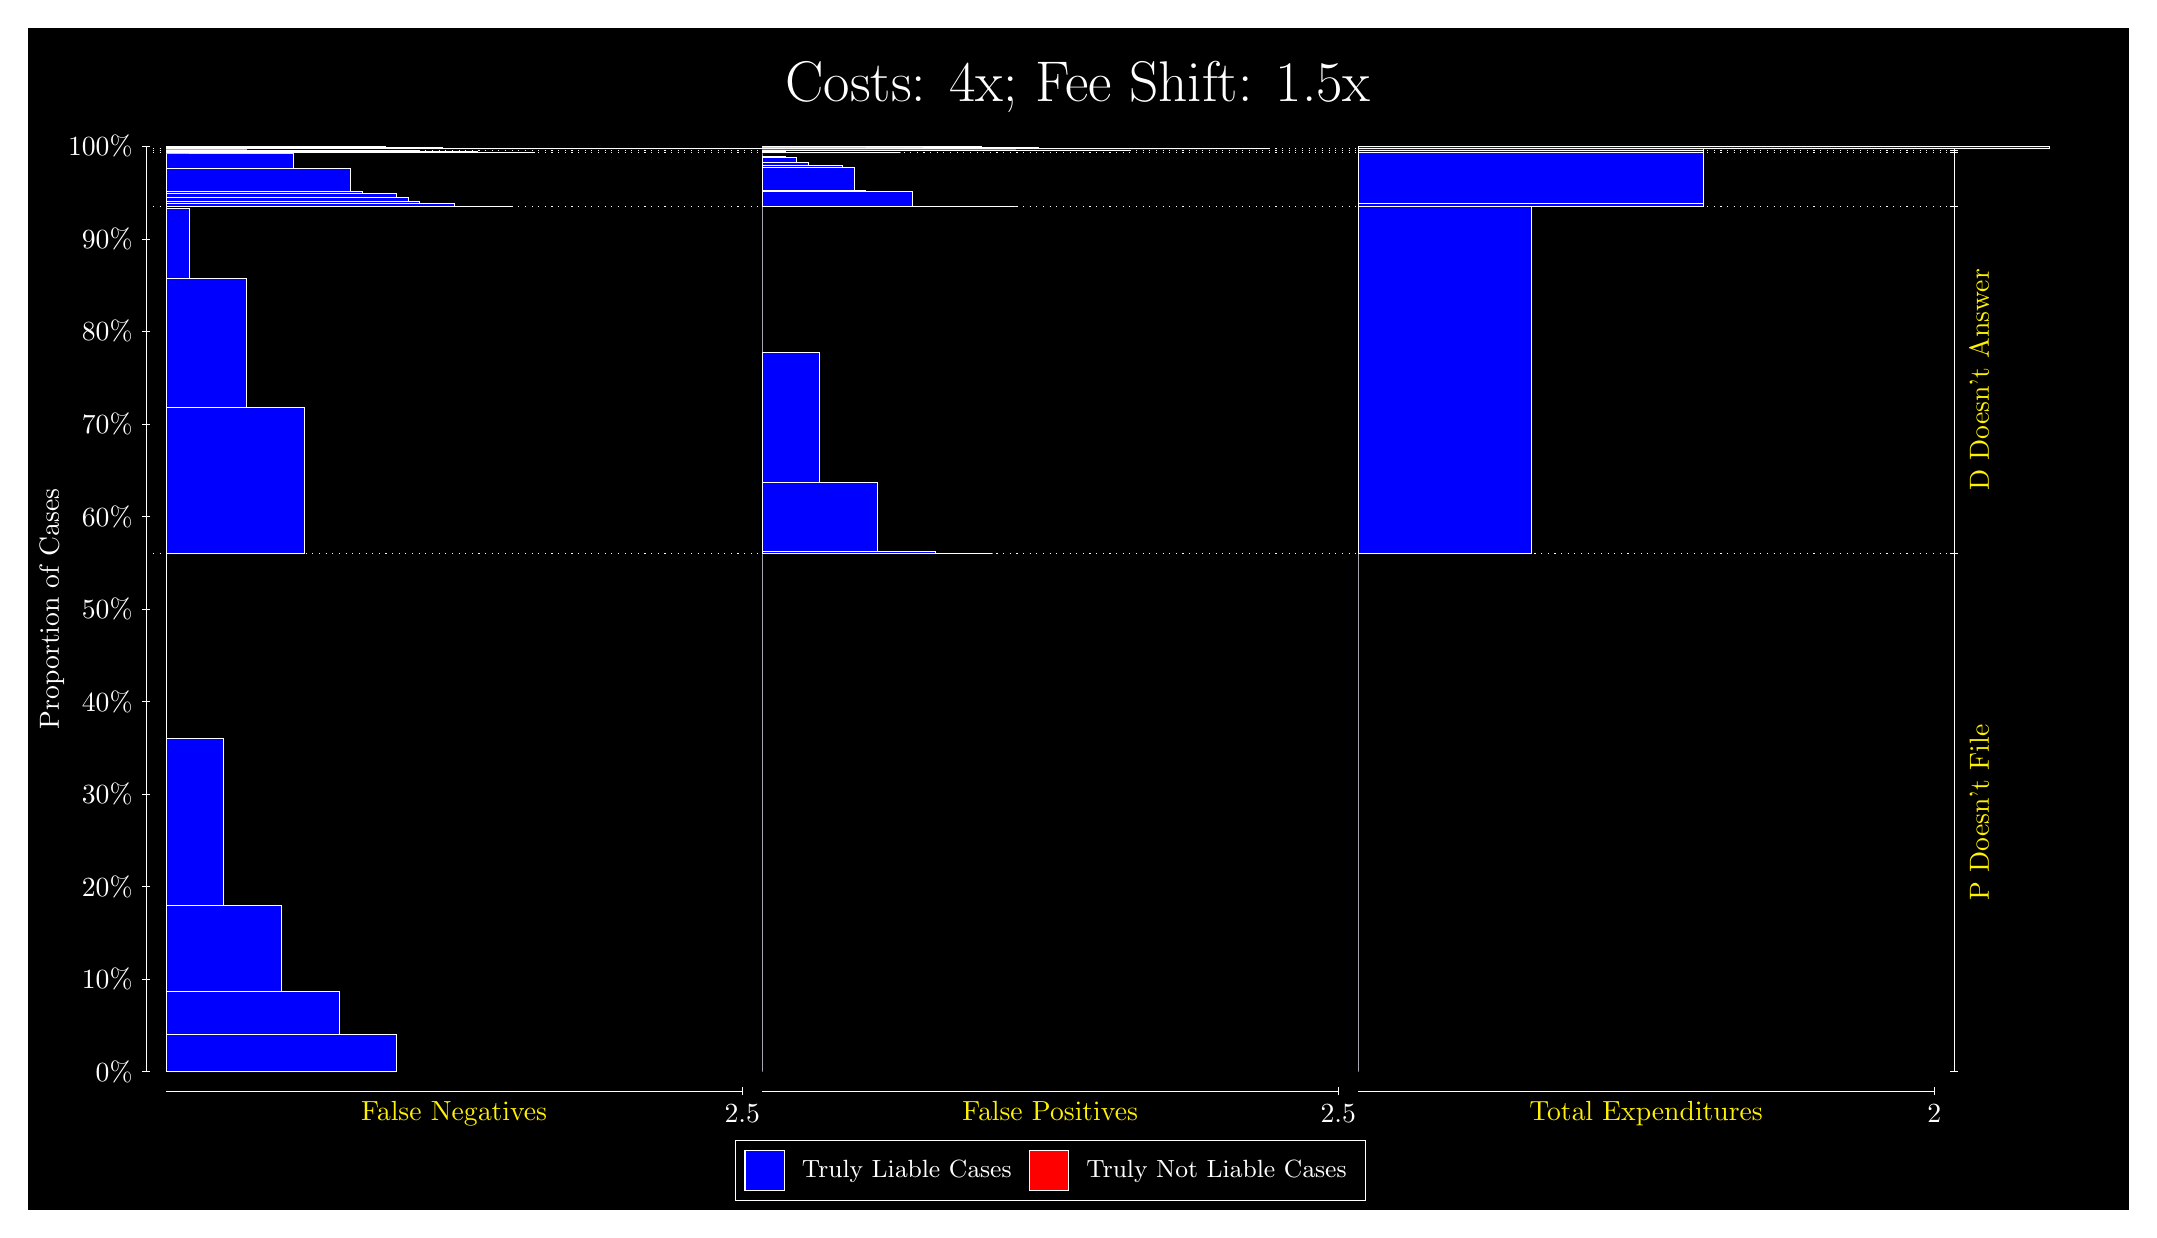
\begin{tikzpicture}
\draw[fill=black] (0,0) rectangle (26.667,15);
\draw[text=white] (0,13.5) rectangle (26.667,15) node[midway] {\huge Costs: 4x; Fee Shift: 1.5x};
\draw[white, very thin] (1.5,1.75) -- (1.5,13.5);
\node[rotate=90, text=white, anchor=center] at (0.3, 7.625) {Proportion of Cases};
\draw[white, very thin] (1.45,1.75) -- (1.55,1.75);
\node[text=white, anchor=east] at (1.45, 1.75) {0\%};
\draw[white, very thin] (1.45,2.925) -- (1.55,2.925);
\node[text=white, anchor=east] at (1.45, 2.925) {10\%};
\draw[white, very thin] (1.45,4.1) -- (1.55,4.1);
\node[text=white, anchor=east] at (1.45, 4.1) {20\%};
\draw[white, very thin] (1.45,5.275) -- (1.55,5.275);
\node[text=white, anchor=east] at (1.45, 5.275) {30\%};
\draw[white, very thin] (1.45,6.45) -- (1.55,6.45);
\node[text=white, anchor=east] at (1.45, 6.45) {40\%};
\draw[white, very thin] (1.45,7.625) -- (1.55,7.625);
\node[text=white, anchor=east] at (1.45, 7.625) {50\%};
\draw[white, very thin] (1.45,8.8) -- (1.55,8.8);
\node[text=white, anchor=east] at (1.45, 8.8) {60\%};
\draw[white, very thin] (1.45,9.975) -- (1.55,9.975);
\node[text=white, anchor=east] at (1.45, 9.975) {70\%};
\draw[white, very thin] (1.45,11.15) -- (1.55,11.15);
\node[text=white, anchor=east] at (1.45, 11.15) {80\%};
\draw[white, very thin] (1.45,12.325) -- (1.55,12.325);
\node[text=white, anchor=east] at (1.45, 12.325) {90\%};
\draw[white, very thin] (1.45,13.5) -- (1.55,13.5);
\node[text=white, anchor=east] at (1.45, 13.5) {100\%};

\draw[white, very thin] (24.457,1.75) -- (24.457,13.5);
\draw[white, very thin] (24.407,1.75) -- (24.507,1.75);
\node[anchor=west] at (24.407, 1.75) {};
\draw[white, very thin] (24.407,8.3296) -- (24.507,8.3296);
\node[anchor=west] at (24.407, 8.3296) {};
\draw[white, very thin] (24.407,12.739) -- (24.507,12.739);
\node[anchor=west] at (24.407, 12.739) {};
\draw[white, very thin] (24.407,13.419) -- (24.507,13.419);
\node[anchor=west] at (24.407, 13.419) {};
\draw[white, very thin] (24.407,13.448) -- (24.507,13.448);
\node[anchor=west] at (24.407, 13.448) {};
\draw[white, very thin] (24.407,13.472) -- (24.507,13.472);
\node[anchor=west] at (24.407, 13.472) {};
\draw[white, very thin] (24.407,13.5) -- (24.507,13.5);
\node[anchor=west] at (24.407, 13.5) {};

\draw[white, very thin, fill=blue] (1.75,1.75) rectangle (4.6775,2.2207);
\draw[white, very thin, fill=blue] (1.75,2.2207) rectangle (3.9457,2.7673);
\draw[white, very thin, fill=blue] (1.75,2.7673) rectangle (3.2138,3.8565);
\draw[white, very thin, fill=blue] (1.75,3.8565) rectangle (2.4819,5.9819);
\draw[white, very thin, fill=red] (1.75,5.9819) rectangle (1.75,5.9819);
\draw[white, very thin, fill=blue] (1.75,5.9819) rectangle (1.75,8.3296);
\draw[white, very thin, fill=blue] (1.75,8.3296) rectangle (3.5065,10.187);
\draw[white, very thin, fill=blue] (1.75,10.187) rectangle (2.7746,11.829);
\draw[white, very thin, fill=blue] (1.75,11.829) rectangle (2.0428,12.709);
\draw[white, very thin, fill=red] (1.75,12.709) rectangle (1.75,12.709);
\draw[white, very thin, fill=blue] (1.75,12.709) rectangle (1.75,12.739);
\draw[white, very thin, fill=blue] (1.75,12.739) rectangle (6.1413,12.739);
\draw[white, very thin, fill=blue] (1.75,12.739) rectangle (5.5558,12.742);
\draw[white, very thin, fill=blue] (1.75,12.742) rectangle (5.4094,12.78);
\draw[white, very thin, fill=blue] (1.75,12.78) rectangle (4.9703,12.797);
\draw[white, very thin, fill=blue] (1.75,12.797) rectangle (4.8239,12.857);
\draw[white, very thin, fill=blue] (1.75,12.857) rectangle (4.6775,12.903);
\draw[white, very thin, fill=blue] (1.75,12.903) rectangle (4.2384,12.928);
\draw[white, very thin, fill=blue] (1.75,12.928) rectangle (4.092,13.222);
\draw[white, very thin, fill=blue] (1.75,13.222) rectangle (3.9457,13.223);
\draw[white, very thin, fill=blue] (1.75,13.223) rectangle (3.5065,13.224);
\draw[white, very thin, fill=blue] (1.75,13.224) rectangle (3.3602,13.417);
\draw[white, very thin, fill=blue] (1.75,13.417) rectangle (3.2138,13.417);
\draw[white, very thin, fill=blue] (1.75,13.417) rectangle (2.7746,13.417);
\draw[white, very thin, fill=blue] (1.75,13.417) rectangle (2.6283,13.419);
\draw[white, very thin, fill=blue] (1.75,13.419) rectangle (2.0428,13.419);
\draw[white, very thin, fill=red] (1.75,13.419) rectangle (1.75,13.419);
\draw[white, very thin, fill=blue] (1.75,13.419) rectangle (6.4341,13.419);
\draw[white, very thin, fill=blue] (1.75,13.419) rectangle (5.7022,13.432);
\draw[white, very thin, fill=blue] (1.75,13.432) rectangle (4.9703,13.448);
\draw[white, very thin, fill=blue] (1.75,13.448) rectangle (4.2384,13.448);
\draw[white, very thin, fill=blue] (1.75,13.448) rectangle (3.5065,13.448);
\draw[white, very thin, fill=red] (1.75,13.448) rectangle (1.75,13.448);
\draw[white, very thin, fill=blue] (1.75,13.448) rectangle (3.5065,13.448);
\draw[white, very thin, fill=blue] (1.75,13.448) rectangle (2.7746,13.463);
\draw[white, very thin, fill=blue] (1.75,13.463) rectangle (2.0428,13.472);
\draw[white, very thin, fill=red] (1.75,13.472) rectangle (1.75,13.472);
\draw[white, very thin, fill=blue] (1.75,13.472) rectangle (1.75,13.472);
\draw[white, very thin, fill=blue] (1.75,13.472) rectangle (13.46,13.472);
\draw[white, very thin, fill=blue] (1.75,13.472) rectangle (12.728,13.472);
\draw[white, very thin, fill=blue] (1.75,13.472) rectangle (11.996,13.472);
\draw[white, very thin, fill=blue] (1.75,13.472) rectangle (11.265,13.476);
\draw[white, very thin, fill=blue] (1.75,13.476) rectangle (10.533,13.476);
\draw[white, very thin, fill=blue] (1.75,13.476) rectangle (9.8008,13.476);
\draw[white, very thin, fill=blue] (1.75,13.476) rectangle (7.4587,13.476);
\draw[white, very thin, fill=blue] (1.75,13.476) rectangle (6.7268,13.476);
\draw[white, very thin, fill=blue] (1.75,13.476) rectangle (5.9949,13.48);
\draw[white, very thin, fill=blue] (1.75,13.48) rectangle (5.2631,13.493);
\draw[white, very thin, fill=blue] (1.75,13.493) rectangle (4.5312,13.5);
\draw[white, very thin, fill=blue] (1.75,13.5) rectangle (3.7993,13.5);
\draw[white, very thin, fill=blue] (1.75,13.5) rectangle (3.0674,13.5);
\draw[white, very thin, fill=blue] (1.75,13.5) rectangle (2.3355,13.5);
\draw[white, very thin, fill=red] (1.75,13.5) rectangle (1.75,13.5);
\draw[white, very thin, fill=red] (9.3189,1.75) rectangle (9.3189,1.75);
\draw[white, very thin, fill=blue] (9.3189,1.75) rectangle (9.3189,8.3296);
\draw[white, very thin, fill=red] (9.3189,8.3296) rectangle (12.246,8.3296);
\draw[white, very thin, fill=blue] (9.3189,8.3296) rectangle (12.246,8.3296);
\draw[white, very thin, fill=blue] (9.3189,8.3296) rectangle (11.515,8.3596);
\draw[white, very thin, fill=blue] (9.3189,8.3596) rectangle (10.783,9.2394);
\draw[white, very thin, fill=blue] (9.3189,9.2394) rectangle (10.051,10.881);
\draw[white, very thin, fill=blue] (9.3189,10.881) rectangle (9.3189,12.739);
\draw[white, very thin, fill=red] (9.3189,12.739) rectangle (12.539,12.739);
\draw[white, very thin, fill=blue] (9.3189,12.739) rectangle (12.539,12.739);
\draw[white, very thin, fill=red] (9.3189,12.739) rectangle (11.954,12.739);
\draw[white, very thin, fill=blue] (9.3189,12.739) rectangle (11.954,12.741);
\draw[white, very thin, fill=blue] (9.3189,12.741) rectangle (11.807,12.741);
\draw[white, very thin, fill=red] (9.3189,12.741) rectangle (11.368,12.741);
\draw[white, very thin, fill=blue] (9.3189,12.741) rectangle (11.368,12.741);
\draw[white, very thin, fill=blue] (9.3189,12.741) rectangle (11.222,12.935);
\draw[white, very thin, fill=blue] (9.3189,12.935) rectangle (11.075,12.935);
\draw[white, very thin, fill=blue] (9.3189,12.935) rectangle (10.636,12.936);
\draw[white, very thin, fill=blue] (9.3189,12.936) rectangle (10.49,13.231);
\draw[white, very thin, fill=blue] (9.3189,13.231) rectangle (10.344,13.255);
\draw[white, very thin, fill=blue] (9.3189,13.255) rectangle (9.9044,13.302);
\draw[white, very thin, fill=blue] (9.3189,13.302) rectangle (9.758,13.361);
\draw[white, very thin, fill=blue] (9.3189,13.361) rectangle (9.6116,13.378);
\draw[white, very thin, fill=blue] (9.3189,13.378) rectangle (9.3189,13.419);
\draw[white, very thin, fill=red] (9.3189,13.419) rectangle (11.075,13.419);
\draw[white, very thin, fill=blue] (9.3189,13.419) rectangle (11.075,13.419);
\draw[white, very thin, fill=blue] (9.3189,13.419) rectangle (10.344,13.419);
\draw[white, very thin, fill=blue] (9.3189,13.419) rectangle (9.6116,13.435);
\draw[white, very thin, fill=blue] (9.3189,13.435) rectangle (9.3189,13.448);
\draw[white, very thin, fill=red] (9.3189,13.448) rectangle (14.003,13.448);
\draw[white, very thin, fill=blue] (9.3189,13.448) rectangle (14.003,13.448);
\draw[white, very thin, fill=blue] (9.3189,13.448) rectangle (13.271,13.448);
\draw[white, very thin, fill=blue] (9.3189,13.448) rectangle (12.539,13.457);
\draw[white, very thin, fill=blue] (9.3189,13.457) rectangle (11.807,13.472);
\draw[white, very thin, fill=blue] (9.3189,13.472) rectangle (11.075,13.472);
\draw[white, very thin, fill=red] (9.3189,13.472) rectangle (15.759,13.472);
\draw[white, very thin, fill=blue] (9.3189,13.472) rectangle (15.759,13.472);
\draw[white, very thin, fill=blue] (9.3189,13.472) rectangle (15.028,13.472);
\draw[white, very thin, fill=red] (9.3189,13.472) rectangle (15.028,13.472);
\draw[white, very thin, fill=blue] (9.3189,13.472) rectangle (15.028,13.472);
\draw[white, very thin, fill=blue] (9.3189,13.472) rectangle (14.296,13.472);
\draw[white, very thin, fill=red] (9.3189,13.472) rectangle (14.296,13.472);
\draw[white, very thin, fill=blue] (9.3189,13.472) rectangle (14.296,13.472);
\draw[white, very thin, fill=blue] (9.3189,13.472) rectangle (13.564,13.475);
\draw[white, very thin, fill=red] (9.3189,13.475) rectangle (13.564,13.475);
\draw[white, very thin, fill=blue] (9.3189,13.475) rectangle (13.564,13.479);
\draw[white, very thin, fill=blue] (9.3189,13.479) rectangle (12.832,13.479);
\draw[white, very thin, fill=blue] (9.3189,13.479) rectangle (12.832,13.493);
\draw[white, very thin, fill=blue] (9.3189,13.493) rectangle (12.1,13.496);
\draw[white, very thin, fill=blue] (9.3189,13.496) rectangle (11.368,13.496);
\draw[white, very thin, fill=blue] (9.3189,13.496) rectangle (10.636,13.496);
\draw[white, very thin, fill=red] (9.3189,13.496) rectangle (9.3189,13.496);
\draw[white, very thin, fill=blue] (9.3189,13.496) rectangle (9.3189,13.5);
\draw[white, very thin, fill=red] (16.888,1.75) rectangle (16.888,1.75);
\draw[white, very thin, fill=blue] (16.888,1.75) rectangle (16.888,8.3296);
\draw[white, very thin, fill=red] (16.888,8.3296) rectangle (19.083,8.3296);
\draw[white, very thin, fill=blue] (16.888,8.3296) rectangle (19.083,12.739);
\draw[white, very thin, fill=red] (16.888,12.739) rectangle (21.279,12.739);
\draw[white, very thin, fill=blue] (16.888,12.739) rectangle (21.279,12.781);
\draw[white, very thin, fill=red] (16.888,12.781) rectangle (21.279,12.781);
\draw[white, very thin, fill=blue] (16.888,12.781) rectangle (21.279,13.419);
\draw[white, very thin, fill=red] (16.888,13.419) rectangle (21.279,13.419);
\draw[white, very thin, fill=blue] (16.888,13.419) rectangle (21.279,13.448);
\draw[white, very thin, fill=red] (16.888,13.448) rectangle (21.279,13.448);
\draw[white, very thin, fill=blue] (16.888,13.448) rectangle (21.279,13.472);
\draw[white, very thin, fill=red] (16.888,13.472) rectangle (25.67,13.472);
\draw[white, very thin, fill=blue] (16.888,13.472) rectangle (25.67,13.48);
\draw[white, very thin, fill=red] (16.888,13.48) rectangle (25.67,13.48);
\draw[white, very thin, fill=blue] (16.888,13.48) rectangle (25.67,13.5);
\draw[white, dotted] (1.5,8.3296) -- (24.457,8.3296);
\draw[white, dotted] (1.5,12.739) -- (24.457,12.739);
\draw[white, dotted] (1.5,13.419) -- (24.457,13.419);
\draw[white, dotted] (1.5,13.448) -- (24.457,13.448);
\draw[white, dotted] (1.5,13.472) -- (24.457,13.472);
\draw[white, very thin] (1.75,1.5) -- (9.0689,1.5);
\node[text=yellow, anchor=north] at (5.4094, 1.5) {False Negatives};
\draw[white, very thin] (9.0689,1.45) -- (9.0689,1.55);
\node[text=white, anchor=north] at (9.0689, 1.45) {2.5};

\draw[white, very thin] (9.3189,1.5) -- (16.638,1.5);
\node[text=yellow, anchor=north] at (12.978, 1.5) {False Positives};
\draw[white, very thin] (16.638,1.45) -- (16.638,1.55);
\node[text=white, anchor=north] at (16.638, 1.45) {2.5};

\draw[white, very thin] (16.888,1.5) -- (24.207,1.5);
\node[text=yellow, anchor=north] at (20.547, 1.5) {Total Expenditures};
\draw[white, very thin] (24.207,1.45) -- (24.207,1.55);
\node[text=white, anchor=north] at (24.207, 1.45) {2};

\node[text=yellow, centered, rotate=90] at (24.777, 5.0398) {P Doesn't File};
\node[text=yellow, centered, rotate=90] at (24.777, 10.534) {D Doesn't Answer};





\draw (12.978300999999998,1.5) node[draw=none] (baseCoordinate) {};
\begin{scope}[align=center]
        \matrix[scale=0.5, draw=white, below=0.5cm of baseCoordinate, nodes={draw}, column sep=0.1cm]{
            \node[rectangle, draw, minimum width=0.5cm, minimum height=0.5cm, fill=blue] {}; &
            \node[draw=none, font=\small, text=white] (B) {Truly Liable Cases}; &
            \node[rectangle, draw, minimum width=0.5cm, minimum height=0.5cm, fill=red] {}; &
            \node[draw=none, font=\small, text=white] (B) {Truly Not Liable Cases}; \\
            };
\end{scope}

\end{tikzpicture}
\end{document}